
\section{Evaluation}\label{sec:eval}

In order to test the efficiency of Dynamic Delay Scheduling, we have designed several 
tests, on both a small and a large scale, using our implementation in Spark, with fair
scheduling enabled. The goal of
these experiments is to demonstrate that an adaptive delay interval provides decreased
job latency in a variety of cluster setups and workloads.

\subsection{Evaluation Setup}
Our small-scale tests were performed on a four node local cluster, with four
task slots (four 1.6 GHz cores for Spark tasks) per machine. All four nodes were
connected through a Gigabit Ethernet switch. The workload chosen for the
small-scale test was an integer sort, on 1GB of input data spread across HDFS.
The main goal behind the small-scale setup is to evaluate our algorithm in a
controlled environment with stable network conditions. To provide data locality
concerns, input data was placed on two nodes, so as to ensure both data-local
and non-local slots for task placement.

In order to have a more realistic evaluation, our large-scale tests were
performed on a 16 node cluster on Amazon EC2, using m3.xlarge instances. The
workload chosen for the large scale test was a TPC-H benchmark (\#7), which
performs a query reading from multiple databases in HDFS, of size ranging from
several megabytes to 80 gigabytes (for a total of ~120GB of input data).
The benchmark is designed to simulate a business query determining the value of
goods shipped between two countries. We chose this particular benchmark because
it consists of a mixture of large and small stages which read from these tables
in parallel. This causes contention for resources in the cluster, creating
situations in which locality and fairness clash. This benchmark also represents
a workload in which fairness is likely to be desired. Without fair sharing,
stages which read from small tables would be significantly delayed by
longer-running stages operating on larger data sets.
All numbers, from both small and large scale, are the average of 3 runs, with
error bars shown.

\subsection{Small Scale Results}
\masoud{@Derek: Argue why sort is a good application for our controlled small
scale eval} The results of our small-scale tests are shown in Figure~\ref{fig:smallscale}.
We performed the sort with the default fixed delay interval (fixed 3 seconds),
with dynamic delay scheduling, and with no delay for comparison. The default of
3 seconds causes a slight increase in completion time (versus no delay). Given
that network conditions were very good between the nodes in the cluster (all
connected to the same switch), having a fixed delay value of 3 seconds causes
increased overhead, because the network overhead of missing locality is far
shorter than 3 seconds. Our adaptive solution performs slightly better, because
the delay interval shrinks based on the feedback from the first round of tasks,
although the job is still too small for there to be the kind of resource
contention that would result in larger speedups. This experiment simply
demonstrates that an incorrect fixed delay interval can actually hurt the
performance of a job, rather than improve it.

\subsection{Large Scale Results}

The results of our large-scale TPC-H tests are shown in Figure~\ref{fig:largescale}, with the same three 
delay setups (fixed 3 seconds, our dynamic solution, and no delay). Even though the default
value still improves completion time versus no delay, the dynamic solution outperforms 
the fixed delay by 15\%. Since the dynamic solution eliminates extraneous
waiting while also still providing an appropriate time to wait for data locality, we see
an improvement over the fixed delay. The improvement is larger than the small-scale for
several reasons. First, with this test being performed in the cloud, network guarantees
are not as strong, creating the need for adaptability if network conditions change. 
Second, with this being a large workload with hundreds of tasks, there is greater 
contention for slots amongst all running stages, creating more opportunity for delay 
scheduling to be applied.

\begin{figure}[t]
    \minipage{0.5\textwidth}
        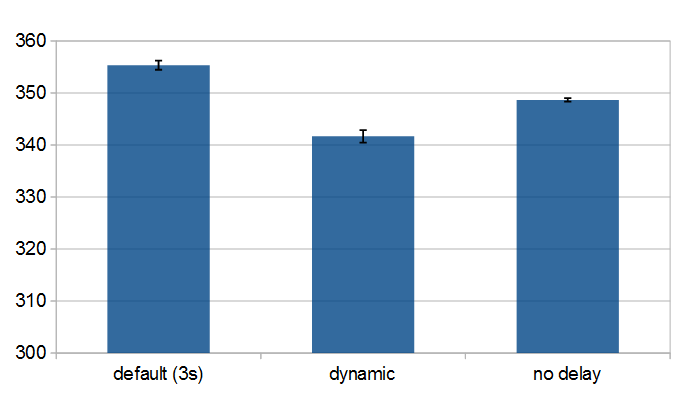
\includegraphics[width=\linewidth]{./smallscale.png}
        \caption{1GB Spark Sort - Job Completion Time (s) vs. Delay Type}
        \label{fig:smallscale}
    \endminipage \hfill
\end{figure}

\begin{figure}[t]
    \minipage{0.5\textwidth}
        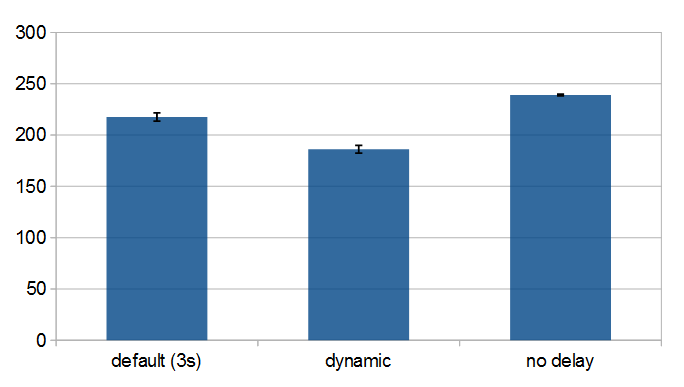
\includegraphics[width=\linewidth]{./largescale.png}
        \caption{120GB Spark TPC-H Query - Job Completion Time (s) vs. Delay Type}
        \label{fig:largescale}
    \endminipage \hfill
\end{figure}

